\section{Breaking Symmetries in 8-connected Grids}
Consider a path which enters an empty room $R$ at some perimeter node $m$ and exits at some other
node $n$ located on the opposite side of the room.
On a 4-connected map we can optimally traverse the room by expanding $m$, following
its macro edge to a node $m'$ on the opposite side of $R$ and finally navigating from $m'$ to $n$.
The length of this path is equal to the Manhattan distance between $m$ and $n$ and thus optimal.
However, if the map consists of 8-connected tiles this strategy is no longer optimal.
In particular, the original (unmodified) map may contain a more direct path to $n$ using one or more diagonal
transtions.
\par
We will address this problem by adding to $R$ a minimal set of additional macro edges
which facilitate optimal traversal between arbitrary pairs of tiles on the perimeter.
Our method is a simple 2 step process (with examples in Figure \ref{fig-macroedges}):
%which we will call the \emph{fan} of $m$ (or simply $\Gamma_{m}$).
%The main idea then is to show that for any pair of tiles appearing on the perimeter of $R$ an optimal length
%path exists which involves only nodes from the perimeter of $R$ and possibly one macro edge.
%Figure \ref{fig-fan} shows some examples of our approach. 
%The method itself is simple:

\begin{enumerate}
\item{First, add a series of macro edges between pairs of perimeter tiles on orthogonal sides of $R$. 
We connect two tiles only if the proposed macro edge represents a path through the interior of $R$ that involves
only diagonal steps. }
\item{Next, add a series of macro edges between pairs of perimeter tiles on opposite sides of $R$.
We connect two tiles only if the proposed macro edge represents a path through the interior of $R$ which is shorter
than any alternative path involving only tiles from the perimeter and possibly one (other) macro edge.
}
\end{enumerate}
%It is easy to see that our method preserves optimality when traversing from some perimeter node $m \in R$ to any other
%perimeter node $n \in R$.
We claim this method preserves optimality when traversing arbitrary rooms in an 8-connected grid map.
\begin{lemma}
Let $R$ be an empty rectangular room in an 8-connected grid map.
Further, let $m$ and $n$ be two locations along its perimeter.
Then, $m$ and $n$ can be connected optimally through a path that mentions only nodes on the perimeter of $R$ and
possibly involves one macro edge.
\end{lemma}

\begin{proof}
There are three cases to consider:
\begin{enumerate}
\item{$m$ and $n$ are on the same side of the perimeter.}
\item{$m$ and $n$ are on orthogonal sides of the perimeter.}
\item{$m$ and $n$ are on opposite sides of the perimeter.}
\end{enumerate}
In the first case we can simply walk along the perimeter from $m$ to $n$; the optimality of this path is immediate. 
In the second and third case we argue as follows: if $m$ and $n$ are not connected by a macro edge
we can walk along the perimeter from $m$ to an intermediate node $m'$ and follow a macro edge to a node $n'$ on the 
same side of the perimeter as $n$. Finally, we walk along the perimeter from $n'$ to $n$.
The length of this path is equal to the octile distance between $m$ and $n$ and therefore optimal
\footnote{Note that in some cases $m' = m$ or $n' = n$ (or both).}.
\end{proof}


\begin{figure}[tb]
       \begin{center}
                       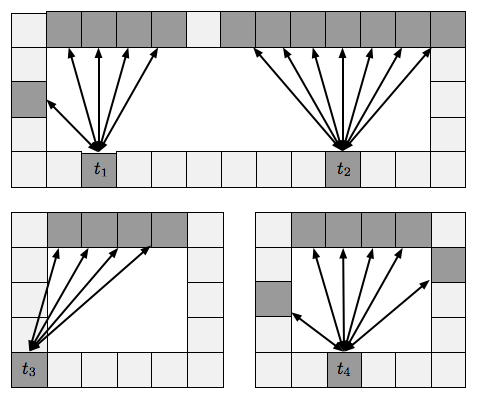
\includegraphics[scale=0.5, trim = 10mm 10mm 10mm 0mm]{diagrams/fan.png}
       \end{center}
	\vspace{-3pt}
       \caption{Some examples.}
       \label{fig-fan}
\end{figure}
